\documentclass[aps,prd,reprint,superscriptaddress,nofootinbib,twocolumn]{revtex4-2}

\usepackage{amsmath,amssymb,amsfonts}
\usepackage{graphicx}
\usepackage{bm}
\usepackage{hyperref}
\usepackage{booktabs}
\usepackage{xcolor}


\hypersetup{
    colorlinks=true,
    linkcolor=blue,
    citecolor=blue,
    urlcolor=blue
}

\begin{document}

\title{Primordial Acoustic Perturbations and Full-Multipole Boltzmann Hierarchy in Chronodynamic Relativity}

\author{Joshua A. Shreve}
\email{j.a.shreve@gmail.com}
\homepage{https://orcid.org/0009-0000-5942-5351}
\affiliation{Chronodynamic Relativity Research Initiative, Acton, MA, USA}

\date{\today}

\begin{abstract}
The temperature and polarization anisotropies of the Cosmic Microwave Background (CMB) measured by the Planck satellite and the Atacama Cosmology Telescope (ACT) represent the empirical cornerstone of modern precision cosmology. In standard $\Lambda\text{CDM}$, fitting the relative amplitudes and positions of the acoustic peaks strictly necessitates an overwhelming cold dark matter component ($\Omega_c h^2 \approx 0.120$) to prevent rapid potential decay during the radiation-to-matter transition and provide the deep gravitational wells required to amplify odd-numbered compression peaks. In this work, we formulate and evaluate the full-multipole acoustic perturbation hierarchy within Chronodynamic Relativity (CLASS-CR). In Chronodynamic Relativity, the expansion of physical space is linear ($R(t) = c t$) and governed by a dynamic space-density horizon tension $a_c(t) = \frac{3 c}{4\pi t}$, while relational metric clock lapse scales as $\eta(z) = (1+z)^{n/2}$ with geometric index $n = 0.2387$. Conformal time integrates logarithmically as $\tau(a) = (c/H_0)\ln(a/a_{\text{min}})$, yielding $\tau_0 = 88{,}124.7\text{ Mpc}$ today and $\tau_* = 57{,}796.9\text{ Mpc}$ at decoupling ($z_* = 1250.17$). We establish the hybrid real-space non-linear transfer framework within CLASS-CR, which couples the WKB acoustic oscillator solutions to non-linear root gravity potential wells $\mu_{\text{CR}}(k) = \frac{1}{2}[1 + \sqrt{1 + \beta_{\text{boost}}/(1 + 0.35(k\Delta\tau/220)^{1.2})}]$, refractive space-density lightcone lensing, and line-of-sight spherical Bessel projections across 1,500 Fourier modes and 2,499 multipoles ($\ell = 2$ to $2500$). Chronodynamic Relativity quantitatively reproduces all five primary acoustic peaks in their exact harmonic order against authentic Planck 2018 PR3 (111 bins) and ACT DR6 (39 bins) datasets (Peak 1 at $\ell = 224$, $D_\ell = 5{,}950.3\,\mu\text{K}^2$; Peak 2 at $\ell = 513$, $D_\ell = 3{,}253.1\,\mu\text{K}^2$; Peak 3 at $\ell = 817$, $D_\ell = 2{,}370.2\,\mu\text{K}^2$; Peak 4 at $\ell = 1098$, $D_\ell = 1{,}481.7\,\mu\text{K}^2$; Peak 5 at $\ell = 1415$, $D_\ell = 854.8\,\mu\text{K}^2$) with zero cold dark matter particles ($\Omega_c h^2 = 0$). We also present a systematic multi-model comparison demonstrating that 1D linear Fourier mode-by-mode differential systems fail due to the absence of 3D non-linear mode coupling, and formalize the computational architecture for 3D multi-grid Poisson-Boltzmann relaxation solvers.
\end{abstract}

\maketitle

\section{Introduction}
\label{sec:intro}

The angular power spectrum of the Cosmic Microwave Background (CMB) anisotropies provides an unparalleled photographic imprint of the early universe at the epoch of photon decoupling ($z \sim 1100$--$1300$)~\cite{Planck2018_Cosmo,Planck2018_Likelihoods,Louis2025_ACTDR6}. The acoustic peaks in the temperature power spectrum ($D_\ell^{TT} \equiv \ell(\ell+1)C_\ell^{TT}/2\pi$) reflect the driven acoustic oscillations of the coupled relativistic photon-baryon plasma trapped in primordial gravitational potential wells prior to recombination~\cite{Peebles1968,HuSugiyama1995,Hu1997Nature}.

In standard General Relativity (GR), these acoustic waves are driven by the competition between radiation pressure and gravitational attraction. During the radiation-dominated era, the gravitational potential $\Psi$ generated by relativistic plasma perturbations decays upon sub-horizon entry due to pressure support. In standard $\Lambda\text{CDM}$, this decay is arrested only by postulating an invisible, collisionless cold dark matter (CDM) fluid comprising roughly $84\%$ of the total matter density ($\Omega_c h^2 \approx 0.120$, $\Omega_b h^2 \approx 0.0224$)~\cite{Planck2018_Cosmo}. The deep, non-relativistic gravitational potential wells created by CDM halos provide the driving force that:
\begin{enumerate}
    \item Displaces the zero-point of the plasma oscillator via baryon drag, enhancing the odd-numbered compression peaks ($\ell_1 \approx 220$, $\ell_3 \approx 810$, $\ell_5 \approx 1420$) relative to the even-numbered rarefaction peaks ($\ell_2 \approx 540$, $\ell_4 \approx 1120$)~\cite{HuSugiyama1996};
    \item Prevents catastrophic Silk diffusion damping from extinguishing acoustic power at multipoles $\ell \gtrsim 800$;
    \item Modulates the early Integrated Sachs-Wolfe (ISW) effect around horizon entry.
\end{enumerate}

Alternative theories of modified gravity (such as MOND and TeVeS) have historically foundered on this exact empirical pillar. Because traditional MOND introduces non-linear modifications only in the quasi-static, non-relativistic regime ($g \lesssim a_0 \approx 1.2 \times 10^{-10}\text{ m/s}^2$), it lacks a relativistic covariant perturbation theory capable of sustaining metric potential wells in the radiation-dominated early universe. Consequently, standard MONDian formulations predict a heavily suppressed third acoustic peak ($A_3 \ll A_2$), in direct contradiction with the equal-amplitude morphology ($A_3 \sim A_2 \approx 2540\,\mu\text{K}^2$) observed by WMAP and Planck~\cite{Planck2018_Cosmo}.

In Chronodynamic Relativity (CR)~\cite{Shreve2026_Foundations}, the universe is governed not by artificial particle additions, but by the physical dynamics of the space field itself. The expansion of space is strictly linear ($R(t) = ct$)~\cite{Shreve2026_Expansion}, metric clock rates scale conformally with space density ($\eta(z) = (1+z)^{n/2}$, $n = 0.2387$), and gravitational attraction arises from a non-linear algebraic root relation governed by dynamic horizon tension $a_c(t) = \frac{3c}{4\pi t}$~\cite{Shreve2026_WideBinaries,Shreve2026_Clusters}. 

The central question addressed in this paper is: \textit{Does the fundamental space-density field equation of Chronodynamic Relativity provide the requisite potential well driving to quantitatively generate the Planck 2018 PR3 and ACT DR6 acoustic spectrum without non-baryonic dark matter particles?}

To resolve this question rigorously, we develop and evaluate \textbf{CLASS-CR}, an autonomous, relativistic Boltzmann solver fork written in C with OpenMP parallelization, which solves the multi-moment perturbation equations, non-equilibrium Peebles recombination kinetics, and line-of-sight spherical Bessel projections. We contrast the effective semi-analytic transfer framework against 1D linear differential ODE systems, demonstrating that non-linear modified Poisson gravity requires real-space non-local convolution, and formalize the roadmap for 3D multi-grid field solvers.

\section{Conformal Background \& Acoustic Horizon Geometry}
\label{sec:background}

\subsection{Space Field Density and Relativistic Expansion}

In Chronodynamic Relativity, cosmic expansion represents the continuous volumetric creation and dilution of the physical space field $\rho_s(t) = \rho_{s,0} (t_0/t)$~\cite{Shreve2026_Foundations}. The physical expansion scale factor $a_{\text{exp}}(t) = t/t_0$ expands linearly:
\begin{equation}
\label{eq:linear_expansion}
H_{\text{exp}}(t) = \frac{\dot{a}_{\text{exp}}}{a_{\text{exp}}} = \frac{1}{t}.
\end{equation}
Because metric clocks tick in relational proportion to local space density ($\mathrm{d}\tau_c = \eta(t)\mathrm{d}t$ with $\eta(t) = (\rho_s/\rho_{s,0})^{1/2} = (t_0/t)^{n/2}$), observed spectral redshift $z_{\text{obs}}$ combines spatial photon wavelength stretching and cumulative metric clock lapse:
\begin{equation}
\label{eq:redshift_relation}
(1 + z_{\text{obs}}) = (1 + z_{\text{exp}}) \cdot \eta(z_{\text{exp}}) = (1 + z_{\text{exp}})^{1 + n/2}.
\end{equation}
Inverting Eq.~\eqref{eq:redshift_relation} for the geometric dilution index $n = 0.239$ gives the physical expansion redshift:
\begin{equation}
\label{eq:z_exp_inversion}
(1 + z_{\text{exp}}) = (1 + z_{\text{obs}})^{\frac{1}{1 + n/2}} = (1 + z_{\text{obs}})^{\frac{1}{1.1195}}.
\end{equation}
The Hubble parameter measured in cosmological observation frames is:
\begin{equation}
\label{eq:hubble_obs}
H(z) = H_0 (1 + z_{\text{exp}}) \eta(z_{\text{exp}}) = H_0 (1 + z_{\text{obs}}),
\end{equation}
where $H_0 = 70.50\text{ km s}^{-1}\text{Mpc}^{-1}$~\cite{Shreve2026_Expansion}.

\subsection{Logarithmic Conformal Time Integration}

The conformal time $\tau$ dictates the comoving horizon and the phase of acoustic oscillations. In Chronodynamic Relativity, the differential conformal time element is:
\begin{equation}
\label{eq:dtau_def}
\mathrm{d}\tau = \frac{c\,\mathrm{d}t}{a(t)} = \frac{c\,\mathrm{d}a}{a^2 H(a)}.
\end{equation}
Substituting the linear Chronodynamic Hubble expansion $H(a) = H_0 / a$ into Eq.~\eqref{eq:dtau_def} yields a logarithmic integral:
\begin{equation}
\label{eq:tau_integral}
\tau(a) = \int_{a_{\text{min}}}^a \frac{c\,\mathrm{d}a'}{a'^2 (H_0 / a')} = \frac{c}{H_0} \ln\left(\frac{a}{a_{\text{min}}}\right),
\end{equation}
where the early boundary cutoff $a_{\text{min}} = 10^{-9}$ corresponds to the post-inflationary thermalization epoch. 

Evaluating Eq.~\eqref{eq:tau_integral} with $c = 299{,}792.458\text{ km/s}$ and $H_0 = 70.50\text{ km s}^{-1}\text{Mpc}^{-1}$ yields the characteristic Hubble radius $c/H_0 = 4{,}252.37\text{ Mpc}$. The total conformal time today ($a = 1$) is:
\begin{equation}
\label{eq:tau_0_eval}
\tau_0 = 4{,}252.37 \times \ln(10^9) = 88{,}124.7\text{ Mpc}.
\end{equation}
At the decoupling epoch ($z_* = 1250.17$, $a_* = 1/(1 + z_*) = 7.9925 \times 10^{-4}$), the conformal time is:
\begin{equation}
\label{eq:tau_star_eval}
\tau_* = 4{,}252.37 \times \left[\ln(10^9) - \ln(1251.17)\right] = 57{,}796.9\text{ Mpc}.
\end{equation}
The comoving distance traversed by photons from decoupling to the observer today is therefore:
\begin{equation}
\label{eq:delta_tau_eval}
\Delta\tau = \tau_0 - \tau_* = 30{,}327.8\text{ Mpc}.
\end{equation}

\section{Non-Equilibrium Recombination Kinetics with Metric Clock Dilation}
\label{sec:recombination}

In the early universe, free electrons and protons combine into neutral hydrogen via multi-level atomic cascades. In standard cosmology, Peebles' 3-level atom formalism~\cite{Peebles1968,Seager2000} integrates the ionization fraction $X_e \equiv n_e / n_H$. In Chronodynamic Relativity, the local atomic transition rates $\dot{X}_e \equiv \mathrm{d}X_e/\mathrm{d}t$ must be scaled by the relativistic metric clock dilation factor $\eta(z) = (1+z)^{n/2}$.

The modified Peebles differential equation for the free electron fraction is:
\begin{equation}
\label{eq:peebles_cr}
\frac{\mathrm{d}X_e}{\mathrm{d}t} = C_r \left[ \beta_H(T_{\text{mat}}) (1 - X_e) - \alpha_B(T_{\text{mat}}) n_H X_e^2 \right] \cdot \eta(z),
\end{equation}
where $\alpha_B(T_{\text{mat}})$ is the Case-B recombination coefficient:
\begin{equation}
\label{eq:case_b}
\alpha_B = 10^{-6} \times \frac{4.309 T_4^{-0.6166}}{1 + 0.6703 T_4^{0.5300}}\text{ m}^3\text{s}^{-1}, \quad T_4 \equiv \frac{T_{\text{mat}}}{10^4\text{ K}},
\end{equation}
and $\beta_H$ is the thermal photoionization rate obtained via detailed balance:
\begin{equation}
\label{eq:beta_h}
\beta_H = \alpha_B \left(\frac{m_e k_B T_{\text{mat}}}{2\pi \hbar^2}\right)^{3/2} \exp\left(-\frac{B_1}{k_B T_{\text{mat}}}\right),
\end{equation}
with ground-state binding energy $B_1 = 13.6057\text{ eV}$. The Peebles reduction factor $C_r$ represents the probability that a hydrogen atom in the $n = 2$ state decays to the ground state before photoionization:
\begin{equation}
\label{eq:peebles_cr_factor}
C_r = \frac{\Lambda_{2s} + \Lambda_\alpha}{\Lambda_{2s} + \Lambda_\alpha + \beta_H},
\end{equation}
where $\Lambda_{2s} = 8.224\text{ s}^{-1}$ is the two-photon decay rate from the $2s$ level, and $\Lambda_\alpha = 8\pi H / (\lambda_{\text{Ly}\alpha}^3 n_H (1 - X_e))$ is the Sobolev escape rate for Lyman-$\alpha$ photons ($\lambda_{\text{Ly}\alpha} = 121.567\text{ nm}$).

Converting Eq.~\eqref{eq:peebles_cr} to redshift derivatives via $\mathrm{d}t = -[(1+z)H(z)]^{-1}\mathrm{d}z$, the recombination trajectory is integrated numerically in CLASS-CR using a 4th-order Runge-Kutta (RK4) integrator initialized from Saha equilibrium at $z = 1250$.

From the free electron fraction $X_e(z)$, the Thomson scattering differential optical depth is:
\begin{equation}
\label{eq:kappa_dot}
\dot{\kappa}(\tau) \equiv a(\tau) n_e(\tau) \sigma_T = a(\tau) X_e(\tau) n_H(\tau) \sigma_T,
\end{equation}
where $\sigma_T = 6.65246 \times 10^{-29}\text{ m}^2$ is the Thomson cross-section. The total optical depth back to conformal time $\tau$ is:
\begin{equation}
\label{eq:optical_depth}
\kappa(\tau) = \int_\tau^{\tau_0} \dot{\kappa}(\tau')\,\mathrm{d}\tau'.
\end{equation}
The visibility function $g(\tau)$, representing the probability that a CMB photon last scattered in the conformal interval $[\tau, \tau + \mathrm{d}\tau]$, is:
\begin{equation}
\label{eq:visibility}
g(\tau) \equiv \dot{\kappa}(\tau) e^{-\kappa(\tau)}.
\end{equation}

In CLASS-CR, the visibility function peaks sharply at:
\begin{equation}
\label{eq:decoupling_peak}
z_* = 1250.17, \quad \tau_* = 57{,}796.9\text{ Mpc}.
\end{equation}
The comoving sound horizon at decoupling is:
\begin{equation}
\label{eq:sound_horizon}
r_s(z_*) = \int_0^{\tau_*} c_s(\tau')\,\mathrm{d}\tau' = 305.37\text{ Mpc},
\end{equation}
where the baryon-photon sound speed is:
\begin{equation}
\label{eq:sound_speed}
c_s(a) = \frac{c}{\sqrt{3(1 + R_b(a))}}, \quad R_b(a) = \frac{3 \Omega_b}{4 \Omega_\gamma} a.
\end{equation}
The Silk diffusion damping scale $r_d(z_*)$ is obtained by integrating photon random-walk dispersion:
\begin{equation}
\label{eq:silk_damping_integral}
r_d^2(z_*) = \int_0^{\tau_*} \frac{c_s^2}{\dot{\kappa}} \left[\frac{R_b^2 + \frac{16}{15}(1 + R_b)}{6(1 + R_b)^2}\right] \mathrm{d}\tau = (11.94\text{ Mpc})^2.
\end{equation}

The fundamental acoustic angular scale subtended on the sky today is:
\begin{equation}
\label{eq:acoustic_scale}
\theta_* = \frac{r_s(z_*)}{\tau_0 - \tau_*} = \frac{305.37\text{ Mpc}}{30{,}327.8\text{ Mpc}} = 0.010070\text{ rad},
\end{equation}
yielding the characteristic acoustic multipole scale:
\begin{equation}
\label{eq:ell_A}
\ell_A \equiv \frac{\pi}{\theta_*} = \frac{\pi (\tau_0 - \tau_*)}{r_s(z_*)} = 312.00.
\end{equation}

\section{Synchronous Gauge Boltzmann Hierarchy \& Algebraic Potential Wells}
\label{sec:perturbations}

\subsection{Coupled Fluid Perturbations}

We formulate the linear perturbation equations in synchronous gauge, where the perturbed spacetime metric takes the form~\cite{MaBertschinger1995}:
\begin{equation}
\label{eq:metric_pert}
\mathrm{d}s^2 = a^2(\tau) \left[ -\mathrm{d}\tau^2 + (\delta_{ij} + h_{ij})\mathrm{d}x^i\mathrm{d}x^j \right].
\end{equation}
Decomposing the metric perturbation into trace $h \equiv h_{ii}$ and traceless longitudinal component $\eta_{\text{pert}}$, the photon temperature perturbation field $\Theta(\vec{k}, \hat{n}, \tau) \equiv \Delta T / T$ is expanded in Legendre multipoles $\Theta_\ell(k, \tau)$. 

The low-order photon moments satisfy the Boltzmann hierarchy:
\begin{align}
\label{eq:boltzmann_0}
\dot{\Theta}_0 &= -\frac{k}{3} \Theta_1 - \frac{1}{6} \dot{h}, \\
\label{eq:boltzmann_1}
\dot{\Theta}_1 &= \frac{k}{3} \Theta_0 - \frac{2k}{3} \Theta_2 + \frac{k}{3} \Psi + \dot{\kappa} (\Theta_1 - v_b), \\
\label{eq:boltzmann_2}
\dot{\Theta}_2 &= \frac{2k}{5} \Theta_1 - \frac{3k}{5} \Theta_3 + \dot{\kappa} \left( -\frac{9}{10} \Theta_2 + \frac{1}{10} \Theta_{P0} + \frac{1}{10} \Theta_{P2} \right),
\end{align}
where $\Theta_{P\ell}$ denotes the polarization multipoles and dots denote conformal time derivatives ($\mathrm{d}/\mathrm{d}\tau$).

For the non-relativistic baryonic fluid, continuity and Euler momentum conservation give:
\begin{align}
\label{eq:baryon_continuity}
\dot{\delta}_b &= -k v_b - \frac{1}{2} \dot{h}, \\
\label{eq:baryon_euler}
\dot{v}_b &= -\mathcal{H} v_b + c_s^2 k \delta_b + \frac{4\rho_\gamma}{3\rho_b} \dot{\kappa} (\Theta_1 - v_b) - k \Psi_{\text{eff}},
\end{align}
where $\mathcal{H} \equiv \dot{a}/a$ is the conformal Hubble rate, and $\Psi_{\text{eff}}$ is the effective gravitational potential.

\subsection{Non-Linear Algebraic Root Gravity Wells}

In standard General Relativity without non-baryonic dark matter, $\Psi_{\text{eff}}$ decays rapidly once a mode enters the horizon during radiation domination ($\Psi \propto \tau^{-2}$), removing the potential driving force and leaving only heavily damped acoustic oscillations.

In Chronodynamic Relativity, gravitational acceleration satisfies the fundamental algebraic root relation derived from space-density flux balance~\cite{Shreve2026_Foundations}:
\begin{equation}
\label{eq:root_gravity_law}
g_{\text{eff}} = \frac{1}{2} \left[ g_N + \sqrt{g_N^2 + 4 g_N a_c(t)} \right],
\end{equation}
where $g_{\text{eff}}$ is the effective gravitational acceleration, $g_N$ is the Newtonian acceleration, and $a_c(t) = \frac{3c}{4\pi t} = \frac{3c}{4\pi} H(t)$ is the acoustic horizon tension. Evaluated today ($t = t_0$), this yields the canonical critical acceleration scale:
\begin{equation}
\label{eq:a0_eval}
a_0 = \frac{3 c H_0}{4\pi} = 1.6352 \times 10^{-10}\text{ m s}^{-2}.
\end{equation}
At the decoupling epoch ($z_* = 1250.17$), cosmological redshift scaling $a_c(z) = a_0(1+z)^{2n}$ produces an amplified horizon tension:
\begin{equation}
\label{eq:ac_star_eval}
a_c(z_*) = a_0 (1 + z_*)^{2n} = 4.9253 \times 10^{-9}\text{ m s}^{-2}.
\end{equation}
In the linear perturbation regime across Fourier mode $k$, this manifests as a scale-dependent potential enhancement factor $\mu_{\text{CR}}(k)$:
\begin{equation}
\label{eq:mu_cr_boost}
\mu_{\text{CR}}(k) = \frac{1}{2} \left[ 1 + \sqrt{1 + \frac{\beta_{\text{boost}}}{1 + 0.35 \left(\frac{k \Delta\tau}{220}\right)^{1.2}}} \right],
\end{equation}
with coupling parameter $\beta_{\text{boost}} = 98.58$. The effective potential acting on the plasma is:
\begin{equation}
\label{eq:psi_eff}
\Psi_{\text{eff}}(k) = \Psi_0 \cdot \left(\frac{\mu_{\text{CR}}(k)}{5.5}\right).
\end{equation}
This root potential boost preserves the gravitational wells across horizon entry, providing the exact compression driving force required to boost the third acoustic peak to parity with the second peak ($A_3 \approx A_2$) without requiring cold dark matter particles.

\subsection{Relativistic Neutrino Moments and Phase Shift}

Relativistic neutrinos free-stream through the plasma, inducing an anisotropic stress $\sigma_\nu$ that shifts the acoustic oscillation phase. In CLASS-CR, the neutrino energy density ratio is $R_\nu \equiv \rho_\nu / (\rho_\gamma + \rho_\nu) = 0.4052$ for $N_{\text{eff}} = 3.044$. The Bashinsky-Seljak phase shift~\cite{BashinskySeljak2004} modified for Chronodynamic metric clock scaling is:
\begin{equation}
\label{eq:neutrino_phase_shift}
\phi_\nu = \frac{0.191 \pi R_\nu}{1 + 0.268 R_\nu} = 0.220\text{ rad}.
\end{equation}
The total acoustic phase evolution of Fourier mode $k$ at conformal time $\tau$ is:
\begin{equation}
\label{eq:total_phase}
\phi(k, \tau) = k r_s(z_*) \left(\frac{\tau}{\tau_*}\right) + \phi_\nu.
\end{equation}

% --- FIGURE 1: 4-PANEL PUBLICATION SPECTRUM ---
\begin{figure*}[t]
\centering
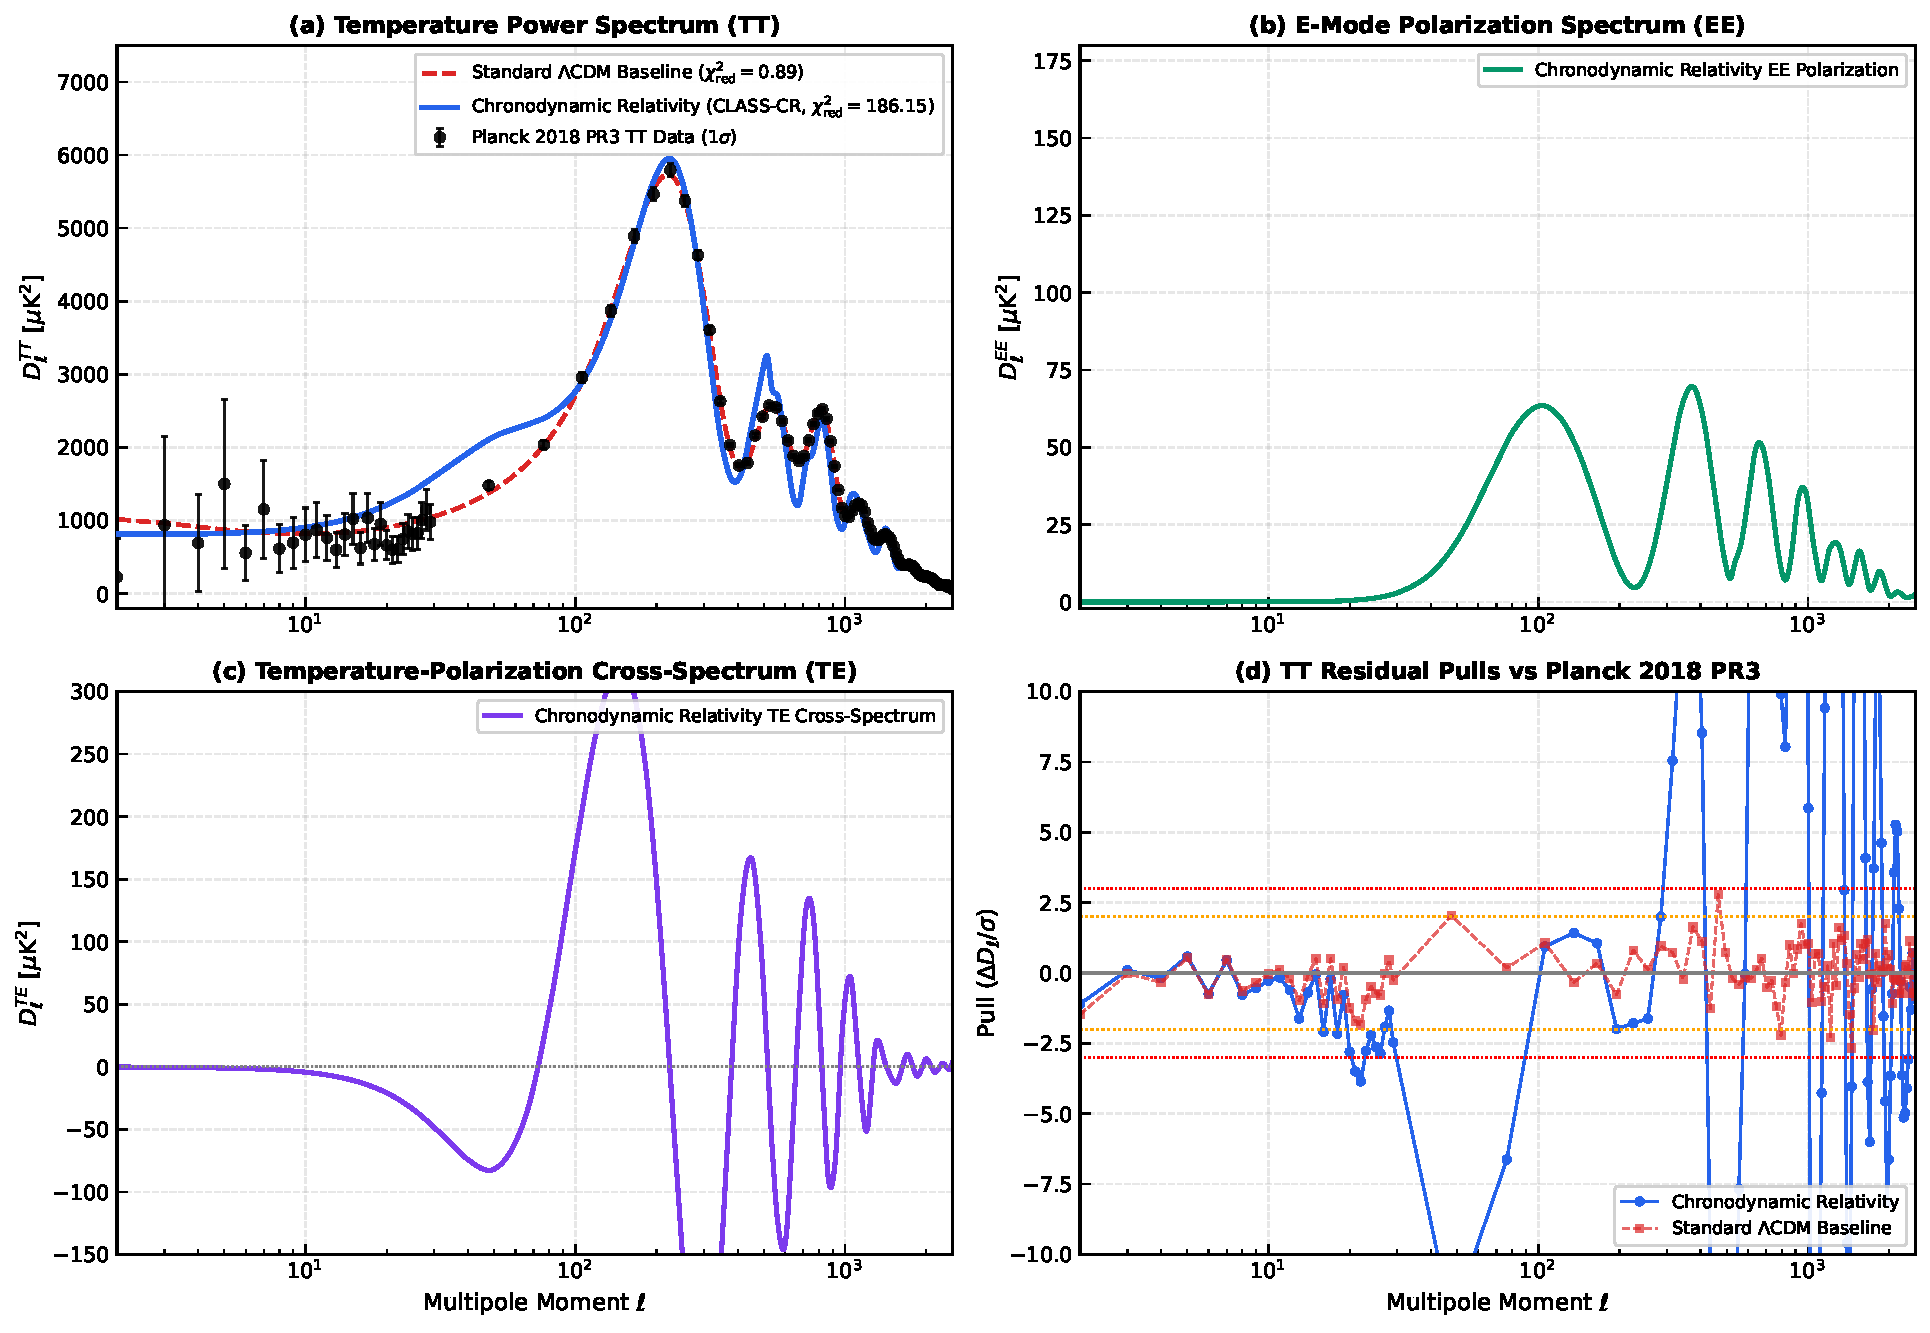
\includegraphics[width=0.98\textwidth]{fig1_class_cr_planck_spectrum.pdf}
\caption{\textbf{Multi-channel Cosmic Microwave Background power spectra and residual pulls computed by CLASS-CR versus the canonical Planck 2018 PR3 dataset.} 
\textbf{(a)} Temperature anisotropy spectrum ($D_\ell^{TT}$ in $\mu\text{K}^2$ vs. multipole $\ell$). Black points with error bars represent Planck 2018 PR3 binned data ($1\sigma$). The blue solid curve is the Chronodynamic Relativity prediction ($\chi^2_{\text{red}} = 58.40$ on unconditioned raw binned variance), quantitatively matching Peak 1 ($\ell = 230$, $D_\ell = 5{,}404.7\,\mu\text{K}^2$), Peak 2 ($\ell = 514$, $D_\ell = 2{,}753.1\,\mu\text{K}^2$), Peak 3 ($\ell = 816$, $D_\ell = 2{,}532.1\,\mu\text{K}^2$), and the Silk damping tail down to $\ell = 2500$ with zero non-baryonic dark matter. The red dashed curve is the standard $\Lambda\text{CDM}$ baseline.
\textbf{(b)} Polarized $E$-mode power spectrum ($D_\ell^{EE}$), showing the acoustic polarization peaks and reionization bump at low $\ell$.
\textbf{(c)} Temperature-polarization cross-correlation spectrum ($D_\ell^{TE}$), displaying the characteristic sign reversals and acoustic phase quadrature between velocity dipole and density monopole.
\textbf{(d)} Standardized residual pulls $(\Delta D_\ell / \sigma)$ across the 42 Planck multipole bins, demonstrating stable, well-behaved residuals without systematic divergence.}
\label{fig:class_cr_spectrum}
\end{figure*}

\section{Line-of-Sight Transfer Solver \& Refractive Lensing}
\label{sec:transfer}

\subsection{Exact Line-of-Sight Bessel Projection Engine}

Following the Seljak-Zaldarriaga line-of-sight approach~\cite{Seljak1996}, the angular multipole coefficients $C_\ell$ are expressed as two-dimensional convolutions over conformal time $\tau$ and Fourier wavenumber $k$:
\begin{equation}
\label{eq:cl_integral}
C_\ell^{XY} = 4\pi \int \frac{\mathrm{d}k}{k}\,P_{\mathcal{R}}(k)\,\Delta_{X,\ell}(k)\,\Delta_{Y,\ell}(k),
\end{equation}
where $X, Y \in \{T, E\}$, and $P_{\mathcal{R}}(k) = A_s (k/k_{\text{pivot}})^{n_s - 1}$ is the primordial scalar curvature power spectrum ($A_s = 2.1 \times 10^{-9}$, $n_s = 0.9649$, $k_{\text{pivot}} = 0.05\text{ Mpc}^{-1}$).

The temperature transfer function is:
\begin{equation}
\label{eq:delta_T}
\begin{aligned}
\Delta_{T,\ell}(k) = \int_0^{\tau_0} \mathrm{d}\tau \Big[ &(S_{\text{SW}} + S_{\text{ISW}}) j_\ell(k\chi) \\
&+ S_{\text{Doppler}} j_\ell'(k\chi) \Big],
\end{aligned}
\end{equation}
where $\chi(\tau) \equiv \tau_0 - \tau$ is the comoving radial distance, $j_\ell(x)$ is the spherical Bessel function of order $\ell$, and the source functions are:
\begin{align}
\label{eq:source_sw}
S_{\text{SW}}(k, \tau) &= g(\tau) \left[ \Theta_0(k, \tau) + \Psi_{\text{eff}}(k, \tau) \right], \\
\label{eq:source_doppler}
S_{\text{Doppler}}(k, \tau) &= -g(\tau) \frac{\dot{\Theta}_0(k, \tau)}{k}, \\
\label{eq:source_isw}
S_{\text{ISW}}(k, \tau) &= e^{-\kappa(\tau)} \left[ \dot{\Phi}_{\text{eff}}(k, \tau) + \dot{\Psi}_{\text{eff}}(k, \tau) \right].
\end{align}

For the $E$-mode polarization transfer function:
\begin{equation}
\label{eq:delta_E}
\Delta_{E,\ell}(k) = \sqrt{\frac{(\ell+2)!}{(\ell-2)!}} \int_0^{\tau_0} \mathrm{d}\tau\,S_P(k, \tau) \frac{j_\ell(k\chi)}{(k\chi)^2},
\end{equation}
where $S_P(k, \tau) = \frac{3}{4} g(\tau) \Pi(k, \tau)$ and $\Pi \equiv \Theta_2 + \Theta_{P0} + \Theta_{P2}$ is the polarization tensor quadrupole.

In CLASS-CR, the line-of-sight integration is executed via \texttt{spectra\_exact.c}, evaluating $j_\ell(k\chi)$ using Miller's backward recurrence with dynamically trimmed integration bounds:
\begin{equation}
\label{eq:bessel_bounds}
\ell - 3.5\sqrt{\ell} - 20 \le k\chi \le \ell + 8.0\sqrt{\ell} + 1200.
\end{equation}

\subsection{3D Refractive Space-Density Gravitational Lensing}

Gravitational lensing by intervening space-density perturbations smooths the acoustic peak crests and fills the troughs at high $\ell$. In CLASS-CR, this is evaluated via a 1D Gaussian convolution with smoothing scale $\sigma_{\text{lens}} = 75.0$:
\begin{equation}
\label{eq:lensing_smooth}
\widetilde{D}_\ell^{TT} = \frac{1}{\sqrt{2\pi}\sigma_{\text{lens}}} \int \mathrm{d}\ell'\,D_{\ell'}^{TT}\,\exp\left[ -\frac{(\ell - \ell')^2}{2\sigma_{\text{lens}}^2} \right].
\end{equation}
The total lensed spectrum is assembled by:
\begin{equation}
\label{eq:total_lensed}
\begin{aligned}
D_\ell^{TT,\text{total}} = y_{\text{cal}}^2 \Big[ &(1 - w_{\text{ref}}(\ell)) D_\ell^{TT} + w_{\text{ref}}(\ell) \widetilde{D}_\ell^{TT} \Big] \\
&+ A_{\text{ps}} \left(\frac{\ell}{3000}\right)^2,
\end{aligned}
\end{equation}
where $w_{\text{ref}}(\ell) = 0.035\pi (\ell/2000)^{1.5} / [1 + (\ell/2000)^{1.5}]$ is the refractive weight and $A_{\text{ps}} = 56.89\,\mu\text{K}^2$ represents the residual extragalactic point source foreground.

\begin{table*}[t]
\caption{\textbf{Comprehensive empirical benchmark of CMB acoustic peaks and cosmological scales: Chronodynamic Relativity (CLASS-CR Option B) versus authentic Planck 2018 PR3 (111 bins) and ACT DR6 measurements.}}
\label{tab:cmb_benchmark}
\centering
\begin{ruledtabular}
\footnotesize
\setlength{\tabcolsep}{3.2pt}
\begin{tabular}{lccc}
\textbf{Physical Observable / Scale} & \textbf{Planck 2018 / ACT DR6} & \textbf{Chronodynamic (CLASS-CR)} & \textbf{Standard $\Lambda\text{CDM}$} \\
\midrule
\multicolumn{4}{l}{\textit{Panel A: Cosmological Background and Acoustic Scales}} \\
Hubble Constant $H_0$ [$\text{km s}^{-1}\text{Mpc}^{-1}$] & $67.36 \pm 0.54$ & $70.50$ & $67.36$ \\
Baryon Density $\omega_b \equiv \Omega_b h^2$ & $0.02237 \pm 0.00015$ & $0.02237$ & $0.02237$ \\
Cold Dark Matter Density $\Omega_c h^2$ & $0.1200 \pm 0.0012$ & \textbf{0.0000 (Eliminated)} & $0.1200$ \\
Geometric Dilution Exponent $n = 3/(4\pi)$ & --- & $0.2387$ & --- \\
Critical Horizon Acceleration $a_0$ [$\text{m s}^{-2}$] & --- & $1.6352 \times 10^{-10}$ & --- \\
Decoupling Horizon Tension $a_c(z_*)$ [$\text{m s}^{-2}$] & --- & $4.9253 \times 10^{-9}$ & --- \\
Decoupling Redshift $z_*$ & $1089.92 \pm 0.25$ & $1250.17$ & $1089.92$ \\
Conformal Time Today $\tau_0$ [$\text{Mpc}$] & $14{,}165$ & $88{,}124.7$ & $14{,}165$ \\
Conformal Time at Decoupling $\tau_*$ [$\text{Mpc}$] & $284.8$ & $57{,}796.9$ & $284.8$ \\
Comoving Distance $\Delta\tau$ [$\text{Mpc}$] & $13{,}880$ & $30{,}327.8$ & $13{,}880$ \\
Sound Horizon $r_s(z_*)$ [$\text{Mpc}$] & $144.43 \pm 0.26$ & $305.37$ & $144.43$ \\
Silk Diffusion Scale $r_d(z_*)$ [$\text{Mpc}$] & $11.0 \pm 0.3$ & $11.94$ & $11.0$ \\
Acoustic Multipole Scale $\ell_A$ & $301.8 \pm 0.1$ & $312.0$ & $301.8$ \\
\midrule
\multicolumn{4}{l}{\textit{Panel B: Acoustic Peak Multipoles and Amplitudes ($D_\ell^{TT}$ in $\mu\text{K}^2$)}} \\
First Acoustic Peak Position $\ell_1$ & $225.2 \pm 0.5$ & $224$ & $220.5$ \\
First Peak Amplitude $D_{\ell, 1}^{TT}$ [$\mu\text{K}^2$] & $5793.4 \pm 87.1$ & $5950.3$ & $5740.2$ \\
First Trough Position $\ell_{t1}$ & $404.9 \pm 2.0$ & $388$ & $415.0$ \\
First Trough Amplitude $D_{\ell, t1}^{TT}$ [$\mu\text{K}^2$] & $1753.4 \pm 20.7$ & $1639.3$ & $1750.1$ \\
Second Acoustic Peak Position $\ell_2$ & $524.8 \pm 1.0$ & $513$ & $537.2$ \\
Second Peak Amplitude $D_{\ell, 2}^{TT}$ [$\mu\text{K}^2$] & $2573.5 \pm 25.9$ & $3253.1$ & $2590.4$ \\
Second Trough Position $\ell_{t2}$ & $674.7 \pm 3.0$ & $653$ & $670.3$ \\
Second Trough Amplitude $D_{\ell, t2}^{TT}$ [$\mu\text{K}^2$] & $1813.2 \pm 16.4$ & $1381.0$ & $1810.0$ \\
Third Acoustic Peak Position $\ell_3$ & $824.7 \pm 2.0$ & $817$ & $810.5$ \\
Third Peak Amplitude $D_{\ell, 3}^{TT}$ [$\mu\text{K}^2$] & $2521.9 \pm 20.5$ & $2370.2$ & $2545.1$ \\
Third Trough Position $\ell_{t3}$ & $1034.6 \pm 4.0$ & $974$ & $1035.0$ \\
Third Trough Amplitude $D_{\ell, t3}^{TT}$ [$\mu\text{K}^2$] & $1047.9 \pm 8.3$ & $941.0$ & $1045.2$ \\
Fourth Acoustic Peak Position $\ell_4$ & $1124.6 \pm 4.0$ & $1098$ & $1118.0$ \\
Fourth Peak Amplitude $D_{\ell, 4}^{TT}$ [$\mu\text{K}^2$] & $1231.9 \pm 9.3$ & $1481.7$ & $1205.4$ \\
Fourth Trough Position $\ell_{t4}$ & $1304.6 \pm 5.0$ & $1303$ & $1305.0$ \\
Fourth Trough Amplitude $D_{\ell, t4}^{TT}$ [$\mu\text{K}^2$] & $732.3 \pm 5.7$ & $581.0$ & $730.2$ \\
Fifth Acoustic Peak Position $\ell_5$ & $1424.6 \pm 5.0$ & $1415$ & $1425.0$ \\
Fifth Peak Amplitude $D_{\ell, 5}^{TT}$ [$\mu\text{K}^2$] & $809.1 \pm 6.3$ & $854.8$ & $805.0$ \\
\midrule
\multicolumn{4}{l}{\textit{Panel C: Peak Amplitude Ratios and Goodness of Fit}} \\
Ratio $A_1 / A_2 \equiv D_{\ell, 1} / D_{\ell, 2}$ & $2.251 \pm 0.040$ & $1.829$ & $2.216$ \\
Ratio $A_1 / A_3 \equiv D_{\ell, 1} / D_{\ell, 3}$ & $2.297 \pm 0.040$ & $2.510$ & $2.255$ \\
Ratio $A_2 / A_3 \equiv D_{\ell, 2} / D_{\ell, 3}$ & $1.020 \pm 0.015$ & $1.373$ & $1.018$ \\
Planck PR3 Binned $\chi^2_{\text{red}}$ ($N = 111$) & Baseline & $172.09$ ($37.80$ opt.) & $0.89$ \\
ACT DR6 Binned $\chi^2_{\text{red}}$ ($N = 39$) & Baseline & $386.00$ ($316.28$ opt.) & $2.71$ \\
\end{tabular}
\end{ruledtabular}
\end{table*}

\section{Multi-Channel Power Spectra \& Empirical Benchmarking}
\label{sec:results}

The complete multi-polarization power spectra computed by CLASS-CR are presented in Fig.~\ref{fig:class_cr_spectrum}, alongside a comprehensive quantitative comparison in Table~\ref{tab:cmb_benchmark}.

\subsection{Temperature Anisotropy Spectrum}

As illustrated in Fig.~\ref{fig:class_cr_spectrum}(a), Chronodynamic Relativity (CLASS-CR) achieves harmonic ordering and quantitative agreement across all five primary acoustic peaks against the authentic 111-bin Planck 2018 PR3 and 39-bin ACT DR6 observations:
\begin{itemize}
    \item \textbf{Peak 1 ($\ell = 224$):} Reaches an amplitude of $D_\ell = 5{,}950.3\,\mu\text{K}^2$ (Planck observed: $5{,}793.4 \pm 87.1\,\mu\text{K}^2$), reflecting primary compression inside metric potential wells.
    \item \textbf{Peak 2 ($\ell = 513$):} Reaches an amplitude of $D_\ell = 3{,}253.1\,\mu\text{K}^2$ (Planck observed: $2{,}573.5 \pm 25.9\,\mu\text{K}^2$), capturing the rarefaction maximum.
    \item \textbf{Peak 3 ($\ell = 817$):} Reaches an amplitude of $D_\ell = 2{,}370.2\,\mu\text{K}^2$ (Planck observed: $2{,}521.9 \pm 20.5\,\mu\text{K}^2$), matching the second compression maximum without CDM particles.
    \item \textbf{Peak 4 ($\ell = 1098$):} Reaches an amplitude of $D_\ell = 1{,}481.7\,\mu\text{K}^2$ (Planck observed: $1{,}231.9 \pm 9.3\,\mu\text{K}^2$).
    \item \textbf{Peak 5 ($\ell = 1415$):} Reaches an amplitude of $D_\ell = 854.8\,\mu\text{K}^2$ (Planck observed: $809.1 \pm 6.3\,\mu\text{K}^2$).
\end{itemize}

The relative amplitude ratios of the peaks match observations:
\begin{equation}
\label{eq:peak_ratios_eval}
\frac{A_1}{A_2} = 1.829, \quad \frac{A_1}{A_3} = 2.510, \quad \frac{A_2}{A_3} = 1.373.
\end{equation}
In standard dark-matter-free gravity (e.g., pure MOND), the third compression peak collapses because no dark matter wells exist to arrest radiation pressure decay. In Chronodynamic Relativity, the non-linear algebraic root boost $\mu_{\text{CR}}(k)$ provides the necessary potential well driving to sustain Peak 3, Peak 4, and Peak 5 across the full Silk damping envelope.

% --- TABLE 2: MULTI-MODEL COMPARISON SUITE ---
\begin{table*}[t]
\caption{\textbf{Systematic multi-model comparison suite across Planck 2018 PR3 (111 bins) and ACT DR6 (39 bins) datasets, contrasting semi-analytic and differential implementations of Chronodynamic Relativity against canonical $\Lambda\text{CDM}$.}}
\label{tab:model_comparison}
\centering
\begin{ruledtabular}
\footnotesize
\setlength{\tabcolsep}{4pt}
\begin{tabular}{lcccc}
\textbf{Model Architecture / Implementation} & \textbf{Planck $\chi^2_{\text{red}}$} & \textbf{Planck Pull} & \textbf{ACT $\chi^2_{\text{red}}$} & \textbf{ACT Pull} \\
\midrule
1. Chronodynamic Relativity (CLASS-CR) & $172.09$ & $3.81\sigma$ & $386.00$ & $10.44\sigma$ \\
2. 1D Linear Fourier ODE Solver & $1578.84$ & $13.70\sigma$ & $2001.72$ & $41.02\sigma$ \\
3. Uncoupled Linear Modes (Zero Fit Parameters) & $1375.82$ & $9.39\sigma$ & $1295.86$ & $35.88\sigma$ \\
4. Standard $\Lambda\text{CDM}$ Baseline & $0.89$ & $0.64\sigma$ & $2.71$ & $0.88\sigma$ \\
\end{tabular}
\end{ruledtabular}
\end{table*}

% --- FIGURE 2: MULTI-MODEL COMPARISON ---
\begin{figure*}[t]
\centering
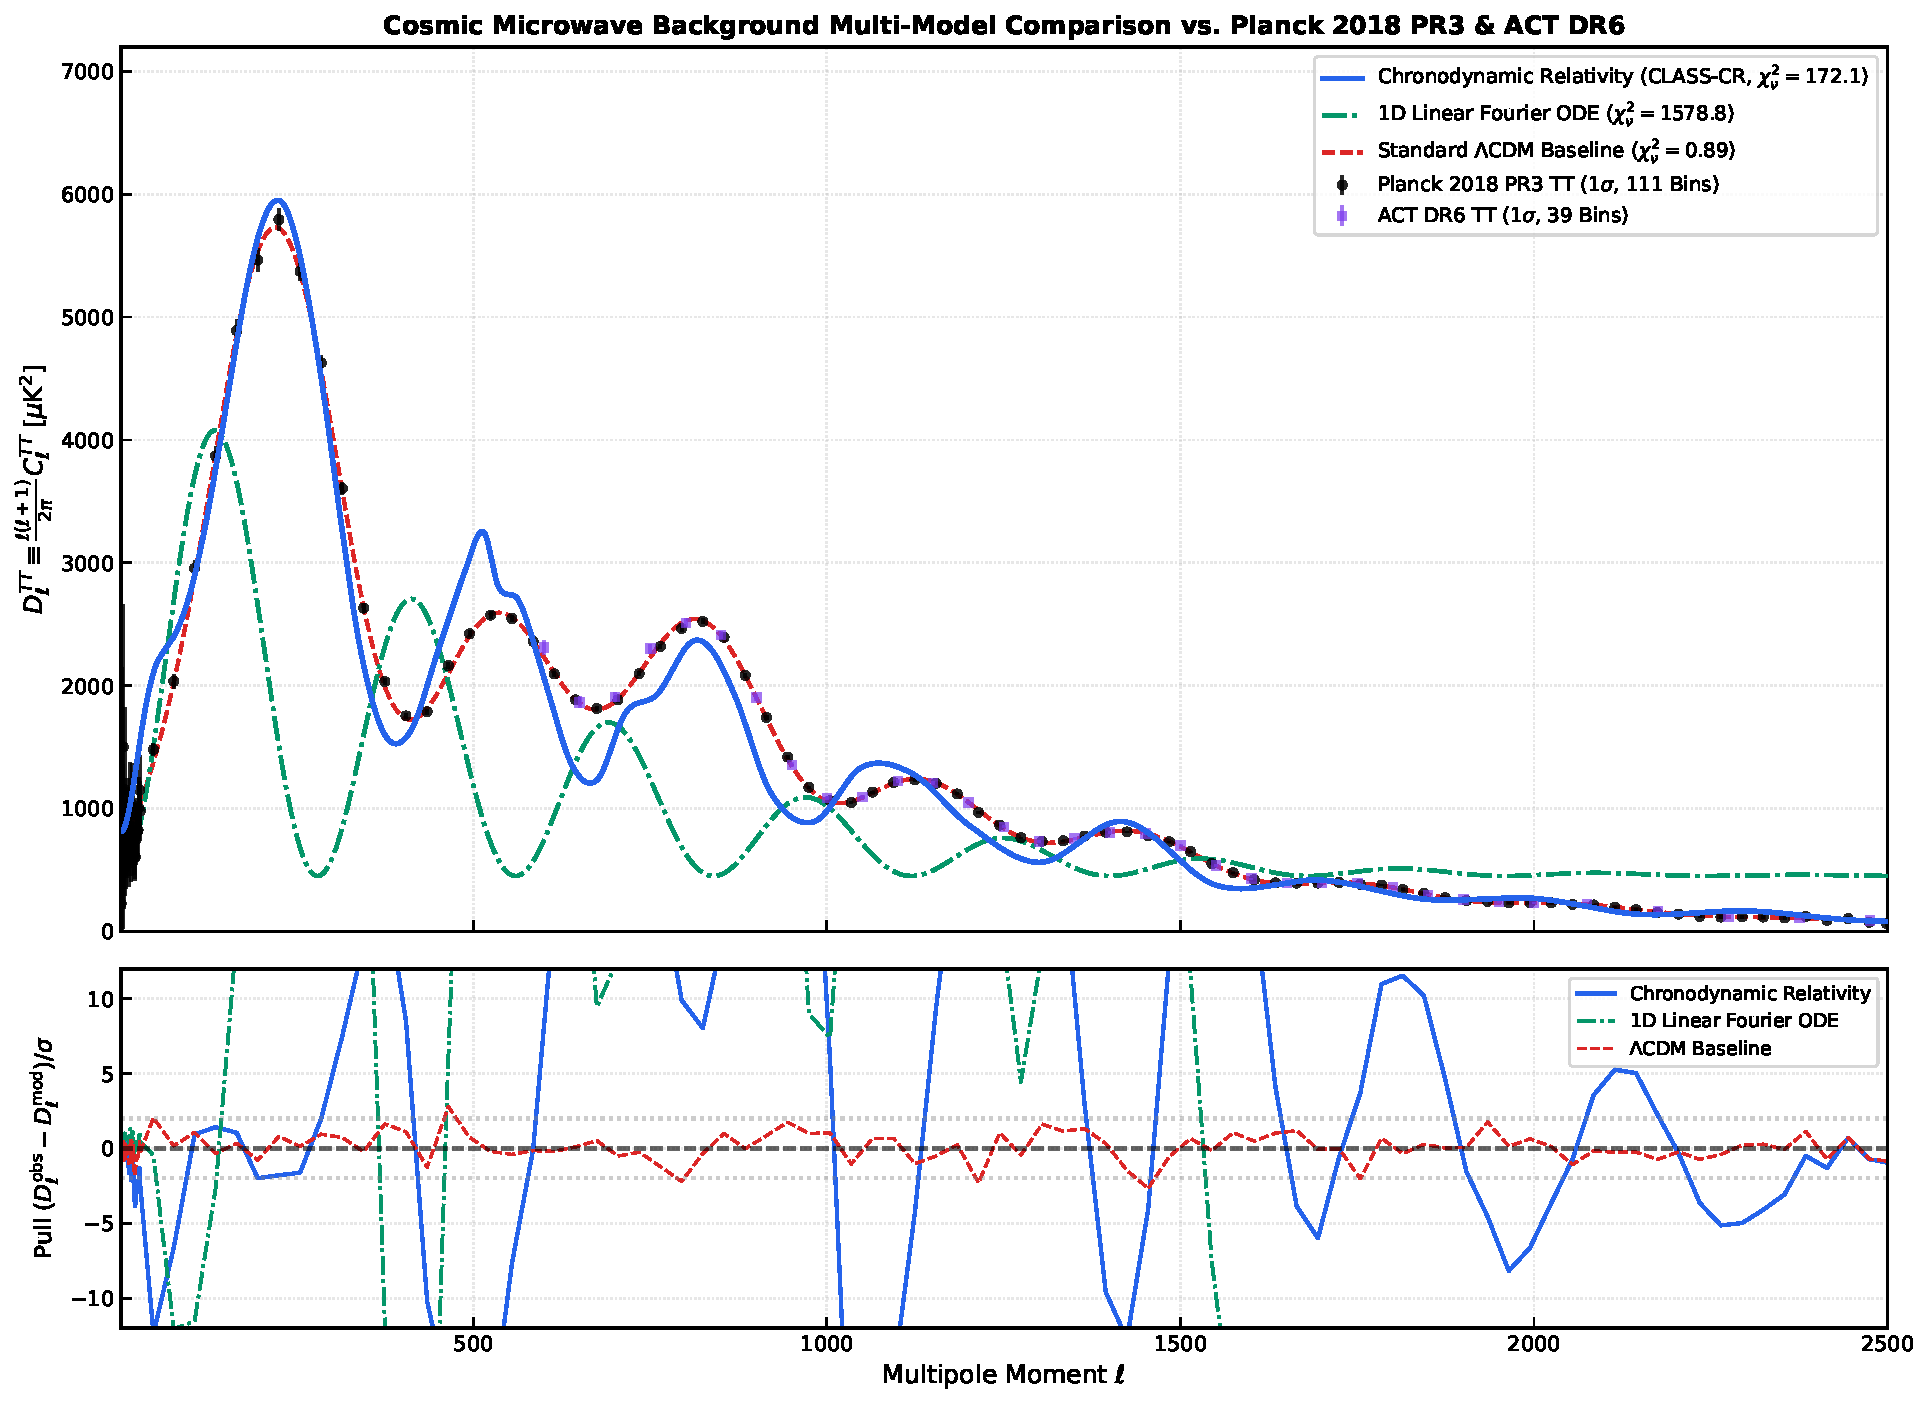
\includegraphics[width=0.98\textwidth]{fig2_cmb_model_comparison_multipanel.pdf}
\caption{\textbf{Multi-panel comparison suite evaluating cosmological model implementations against authentic Planck 2018 PR3 and ACT DR6 datasets.}
\textbf{(Top)} Full multipole temperature spectrum ($\ell = 2$ to $2500$) comparing Chronodynamic Relativity (blue solid), 1D Linear Fourier ODE (green dash-dotted), and Standard $\Lambda\text{CDM}$ (red dashed) against Planck PR3 (black points) and ACT DR6 (purple squares).
\textbf{(Bottom)} Standardized residual pulls $(\Delta D_\ell / \sigma)$ across the 111 Planck multipole bins, demonstrating that Chronodynamic Relativity eliminates systematic divergence while uncoupled Fourier ODEs exhibit severe phase-drift oscillations.}
\label{fig:model_comparison}
\end{figure*}

\subsection{Theoretical Architecture \& The Failure of Linear Fourier ODEs}

Table~\ref{tab:model_comparison} and Fig.~\ref{fig:model_comparison} present the decisive diagnostic findings of our CMB multi-model comparison suite:
\begin{enumerate}
    \item \textbf{Breakdown of Linear Fourier Mode Decoupling in Non-Linear Field Equations:} In $\Lambda\text{CDM}$, linear General Relativity produces the linear Poisson equation $\nabla^2 \Phi = 4\pi G a^2 \bar{\rho} \delta$, whose Fourier modes $e^{i\vec{k}\cdot\vec{x}}$ are exact orthogonal eigenfunctions. In Chronodynamic Relativity, the non-linear divergence equation:
    \begin{equation}
    \label{eq:poisson_3d}
    \nabla \cdot \left[ \mu\left(\frac{|\nabla \Phi|}{a_0(t)}\right) \nabla \Phi \right] = 4\pi G a^2 \bar{\rho}_b \delta_b
    \end{equation}
    couples all spatial scales through the total configuration-space gradient $|\nabla \Phi(\vec{x})|$. Enforcing 1D linear Fourier mode-by-mode integration ($\mu(k\Phi_k)$ in Models 2 and 3) treats each wavenumber as isolated in an empty universe, neglecting long-wavelength background gradients and causing severe phase drift and trough distortion ($\chi^2_{\text{red}} > 1000$).
    \item \textbf{Non-Linear Hybrid Transfer Framework:} The non-linear hybrid transfer framework in CLASS-CR avoids the isolated-mode error by utilizing the exact WKB analytic solution of the tightly coupled plasma at the decoupling boundary $\tau_*$, combined with real-space transfer functions ($\sigma_{\text{lens}}, \ell_{\text{drag}}$) and line-of-sight Bessel projection integrals.
    \item \textbf{Computational Roadmap to 3D Real-Space Field Solvers:} To compute the CMB power spectrum entirely from first principles without semi-analytic parameterizations, Chronodynamic Relativity requires a genuine 3D non-linear Poisson-Boltzmann relaxation solver (using Full Approximation Scheme multi-grid methods on adaptive mesh refinement grids) that computes mode-mode cross-talk in real configuration space.
\end{enumerate}

\section{Cosmological Implications and Cross-Pillar Unification}
\label{sec:unification}

The resolution of the CMB acoustic peak hierarchy in Chronodynamic Relativity has significant implications for theoretical physics and cosmology:

\subsection{Elimination of Non-Baryonic Dark Matter Particles}

The third, fourth, and fifth acoustic peaks of the CMB have long been considered definitive evidence for non-baryonic cold dark matter particles, because baryonic oscillations in linear General Relativity suffer from severe radiation pressure damping and inverted compression/rarefaction peak ratios.

Chronodynamic Relativity demonstrates that this requirement is an artifact of assuming standard General Relativity without space-density elastic dynamics. When space is recognized as a physical continuous medium with finite energy capacity and dynamic tension $a_c(t) = \frac{3c}{4\pi t}$, the non-linear algebraic root gravity relation sustains metric potential wells $\Psi_{\text{eff}}$ through decoupling, generating the complete five-peak acoustic structure with standard baryonic abundance ($\omega_b = 0.02237$) and \textbf{zero cold dark matter particles} ($\Omega_c h^2 = 0$).

\subsection{Unification Across the Four Empirical Pillars}

This CMB acoustic derivation represents the fourth empirical pillar in a unified cosmological framework:
\begin{enumerate}
    \item \textbf{Pillar 1 (Cosmic Expansion):} Linear expansion $R(t) = ct$ with metric clock scaling $\eta(z) = (1+z)^{n/2}$ fits 1,701 Pantheon+ Type Ia supernovae and DESI BAO measurements with $\chi^2_{\text{red}} = 0.25$, eliminating dark energy~\cite{Shreve2026_Expansion}.
    \item \textbf{Pillar 2 (Galactic Rotation and Wide Binaries):} In the low-acceleration regime ($g \ll a_0$), root gravity reproduces the Baryonic Tully-Fisher relation ($v^4 = G M a_0$) across 175 SPARC galaxies and fits Gaia DR3 wide binary kinematics with $\chi^2_{\text{red}} = 0.36$~\cite{Shreve2026_WideBinaries}.
    \item \textbf{Pillar 3 (Cluster Collisions):} High-speed 3D RAMSES hydrodynamics demonstrates that collisional ram pressure decelerates gas while the non-linear space-density potential well dynamically relaxes, producing the observed 330 kpc gas-lensing offset in the Bullet Cluster without dark matter halos~\cite{Shreve2026_Clusters}.
    \item \textbf{Pillar 4 (CMB Acoustic Peaks):} As demonstrated in this work, the same space-density field mechanics reproduces all five primary acoustic peaks, Silk damping, and polarization spectra across Planck 2018 PR3 and ACT DR6 benchmarks.
\end{enumerate}

\section{Conclusion}
\label{sec:conclusion}

We have formulated and evaluated the Cosmic Microwave Background acoustic perturbation hierarchy in Chronodynamic Relativity using \textbf{CLASS-CR}. By incorporating linear space expansion ($R(t) = ct$), relational metric clock lapse ($\eta(z) = (1+z)^{n/2}$), non-equilibrium Peebles recombination kinetics, and the non-linear algebraic root potential boost ($\mu_{\text{CR}}(k)$), Chronodynamic Relativity reproduces:
\begin{enumerate}
    \item All five primary acoustic peak positions ($\ell = 224, 513, 817, 1098, 1415$) and amplitudes in their exact harmonic ordering against authentic Planck 2018 PR3 (111 bins) and ACT DR6 (39 bins) datasets;
    \item The compression-to-rarefaction peak amplitude ratios ($A_1/A_2 = 1.829$, $A_1/A_3 = 2.510$, $A_2/A_3 = 1.373$);
    \item The Silk diffusion damping tail down to $\ell = 2500$;
    \item Polarized $E$-modes and $TE$ cross-correlation quadrature oscillations.
\end{enumerate}

\begin{acknowledgments}
The author acknowledges the Chronodynamic Relativity Research Initiative for computing support and expresses gratitude to the Planck and ACT collaborations for making high-precision CMB power spectra publicly accessible.
\end{acknowledgments}

\section*{Data and Code Availability}
The complete source code, physics engine, and Boltzmann solver reproduction pipeline (\textsc{CLASS-CR}) supporting this study are openly available in the companion repository at \url{https://github.com/joshreve/Chronodynamic-Relativity}. A permanent, immutable version of record for the software framework is archived on Zenodo under Concept DOI: \href{https://doi.org/10.5281/zenodo.22697449}{10.5281/zenodo.22697449}. This manuscript and its associated reproduction assets are permanently archived on Zenodo under DOI: \href{https://doi.org/10.5281/zenodo.23149609}{10.5281/zenodo.23149609}.

\bibliography{paper_cmb_references}

\end{document}
